\chapter{测量时间}\label{ch:g2:measuring-time}

“就再玩五分钟！”——可这到底是多久呢？时间
看不见，摸不着，也不能放在尺子上量。然而我们每天都在\omterm{def:g2:measuring-length:measure}{测量}它：
比赛有胜负，蛋糕不生不焦，
放学铃也准时响起。让我们来学习时间是如何被“驯服”的。

\section{时刻与时长}

\begin{example}[一天的顺序]\label{ex:g2:measuring-time:order}
一天就是一连串依次出现的活动：起床、吃早饭、
上学、吃午饭、下午、吃晚饭、睡觉。“早饭在上学
\emph{之前}”，“晚饭在午饭\emph{之后}”——
“之前”和“之后”是最早学会的时间词，正如“更长”和
“更短”是最早学会的长度词一样。
\end{example}

\begin{omfigure}
\begin{tikzpicture}[scale=0.85]
  \draw[-Stealth, very thick] (0,0) -- (11.4,0);
  \foreach \x/\name in {0.8/起床, 2.9/早饭, 5.0/上学,
      7.1/午饭, 9.2/晚饭, 10.7/睡觉} {
    \fill[omDef] (\x,0) circle (2.4pt);
    \node[above, font=\small, rotate=40, anchor=south west]
      at (\x,0.15) {\name};
  }
\end{tikzpicture}

{\small 一天像数轴一样排开：每件事都有自己的位置，
箭头指示时间的流向——永远向前。}
\end{omfigure}

\begin{definition}[时长]\label{def:g2:measuring-time:duration}
\emph{时刻}\index{时刻}是一天中的一个点，即铃声响起的
那一刻。\emph{时长}\index{时长}是两个时刻之间的一段时间：
从铃声响起到下课结束。时刻回答“\emph{何时}？”，
时长回答“\emph{多久}？”。
\end{definition}

\begin{example}[何时还是多久？]\label{ex:g2:measuring-time:whenhowlong}
“电影在晚饭后开始”说的是\omterm{def:g2:measuring-time:duration}{时刻}。“电影
持续的时间和两个午休一样长”说的是\omterm{def:g2:measuring-time:duration}{时长}。“我
的生日在春天”：\omterm{def:g2:measuring-time:duration}{时刻}。“假期感觉好短”：
\omterm{def:g2:measuring-time:duration}{时长}——本章主要讲的正是\omterm{def:g2:measuring-time:duration}{时长}。
\end{example}

\section{比较时长}

\begin{method}[时长的公平赛跑]\label{met:g2:measuring-time:race}
要判断两件事哪一件持续得更久：
\begin{enumerate}
  \item 让两件事在\emph{同一\omterm{def:g2:measuring-time:duration}{时刻}}开始——“预备，开始！”；
  \item 看哪一件先结束；
  \item 另一件结束时仍在进行的那一件持续得更久。
\end{enumerate}
若两件事不能同时进行（比如今天的洗澡和昨天的晚饭），
就让它们各自和\emph{同一件}第三样东西比一比——
那就是沙漏。
\end{method}

\begin{example}[沙漏]\label{ex:g2:measuring-time:sandtimer}
沙漏是一个中间细窄的小玻璃瓶：沙子
总是需要\emph{同样}长的时间才能漏完。因此它是一位
“裁判”。刷牙时与沙漏比一比：沙子先漏完了——
请刷得更久一点！唱歌与沙漏比一比：歌赢了。因此
这首歌比刷牙持续得更久，虽然它们从未直接
比赛过。
\end{example}

\begin{omfigure}
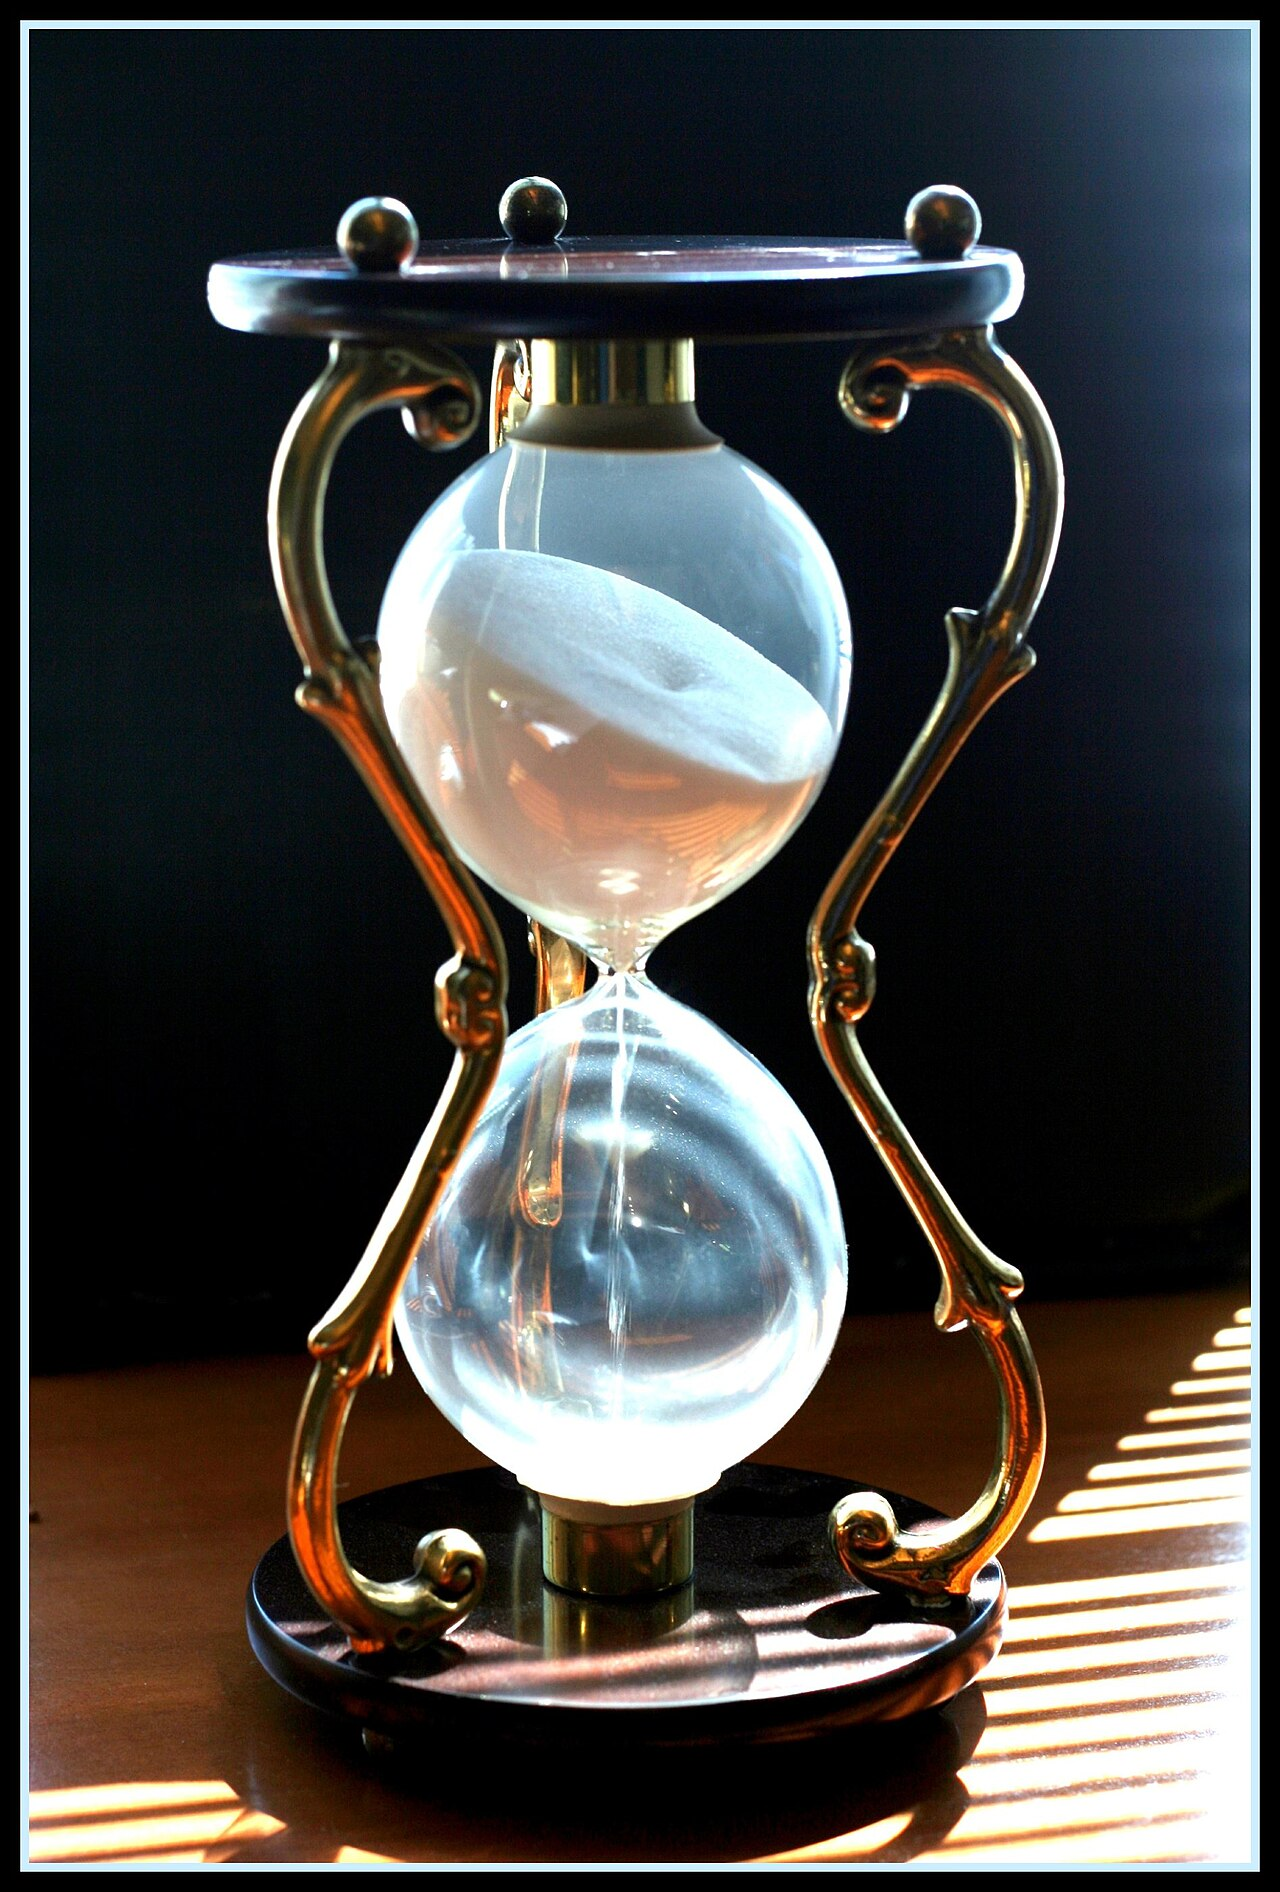
\includegraphics[width=0.34\linewidth]{images/book1/hourglass.jpg}

{\small 沙漏：一段可以握在手中的\omterm{def:g2:measuring-time:duration}{时长}。
沙子总是需要相同的时间穿过中间的细腰——
把它翻过来，它又开始当裁判。\emph{照片：John Morgan，
CC BY 2.0。}}
\end{omfigure}

\begin{remark}[感觉是不准的钟表]\label{rem:g2:measuring-time:feelings}
快乐的下午一晃而过，无聊的队伍慢慢爬——可钟表
对两者的计时可能完全一样。我们对时间的感觉很容易被欺骗，正如
触觉也会对冷热产生误判。这正是像沙漏这样的
“裁判”如此重要的原因：沙子不会觉得无聊。
\end{remark}

\section{数一数稳定的节拍}

\begin{definition}[秒]\label{def:g2:measuring-time:second}
\emph{秒}\index{秒}是全世界通用的时间\omterm{def:g2:measuring-length:measure}{单位}，
记作\unit{s}。一秒钟大约是一次平稳的心跳，
或者大钟表平稳的滴答声。说“一只小鳄鱼，
两只小鳄鱼”，平稳地数下去，大约每数一只
就是一秒。
\end{definition}

\begin{example}[试一试：要用几秒？]\label{ex:g2:measuring-time:count}
请平稳地数秒，同时：舒舒服服地憋住呼吸；水龙头
往杯子里注水；朋友跑到篱笆那里再跑回来。杯子
可能需要 $6$ 秒，跑步需要 $20$ 秒。现在，刷牙和
前面的歌也能得到\emph{数字}——和长度一样，数字
也能被传递，也能被核对。
\end{example}

\begin{example}[钟面上的时间]\label{ex:g2:measuring-time:clock}
秒适合计量短的时间。较长的时间用
\emph{小时}\index{小时}来计：上学的早晨持续好几个\omterm{ex:g2:measuring-time:clock}{小时}，一夜的
睡眠也是如此。钟表的短针指向\omterm{ex:g2:measuring-time:clock}{小时}：正对着
$3$，就是三点整；在 $3$ 和 $4$ 之间，长针
竖直朝下，就是三点半。一整天加上一整夜
一共有 $24$ 个\omterm{ex:g2:measuring-time:clock}{小时}——别忘了，这正是地球
自转一周所需的时间。
\end{example}

\begin{omfigure}
\begin{tikzpicture}[scale=0.85]
  \draw[thick] (0,0) circle (1.5);
  \foreach \h in {1,...,12} {
    \node[font=\footnotesize] at ({90-\h*30}:1.22) {\h};
  }
  \draw[very thick, omDef] (0,0) -- ({90-3*30}:0.8);
  \draw[thick, omThm] (0,0) -- (90:1.05);
  \node[below, font=\small] at (0,-1.75) {三点整};
  \begin{scope}[xshift=6cm]
    \draw[thick] (0,0) circle (1.5);
    \foreach \h in {1,...,12} {
      \node[font=\footnotesize] at ({90-\h*30}:1.22) {\h};
    }
    \draw[very thick, omDef] (0,0) -- ({90-3.5*30}:0.8);
    \draw[thick, omThm] (0,0) -- (270:1.05);
    \node[below, font=\small] at (0,-1.75) {三点半};
  \end{scope}
\end{tikzpicture}

{\small 两个钟面：短针指示\omterm{ex:g2:measuring-time:clock}{小时}。三点半时，
短针已从 $3$ 向 $4$ 走了一半。}
\end{omfigure}

\section{练习}

\begin{exercise}[$\star$]\label{exo:g2:measuring-time:1}
将下列活动按先后排序：晚饭；\ 起床；\ 下午的游戏时间；\ 早饭；
\ 上床睡觉。
\end{exercise}

\begin{exercise}[$\star$]\label{exo:g2:measuring-time:2}
判断下列各句说的是\omterm{def:g2:measuring-time:duration}{时刻}还是\omterm{def:g2:measuring-time:duration}{时长}：“铃声在中午响起”；\ “蛋糕烤
了半个\omterm{ex:g2:measuring-time:clock}{小时}”；\ “我们午饭后离开”；\ “这次旅行感觉
没有尽头”。
\end{exercise}

\begin{exercise}[$\star$]\label{exo:g2:measuring-time:3}
两根蜡烛在同一\omterm{def:g2:measuring-time:duration}{时刻}点燃；红色的那根熄灭时，
蓝色的那根仍在燃烧。哪根蜡烛持续的时间更长？
两根蜡烛遵循了\cref{met:g2:measuring-time:race}中的哪条规则？
\end{exercise}

\begin{exercise}[$\star$]\label{exo:g2:measuring-time:4}
为什么沙漏能公平地判断\omterm{def:g2:measuring-time:duration}{时长}？每次翻转沙漏时，
它有哪一点总是相同的？
\end{exercise}

\begin{exercise}[$\star$]\label{exo:g2:measuring-time:5}
本说，他在牙医那里的枯燥等待持续了“永远”。
他的手表却显示，等待的时间比他最喜欢的动画片还短。这怎么
可能？（见\cref{rem:g2:measuring-time:feelings}。）
\end{exercise}

\begin{exercise}[$\star$]\label{exo:g2:measuring-time:6}
请匀速数秒并\omterm{def:g2:measuring-length:measure}{测量}：写下你的全名
需要多少秒？穿上鞋子需要多少秒？
\end{exercise}

\begin{exercise}[$\star$]\label{exo:g2:measuring-time:7}
秒和\omterm{ex:g2:measuring-time:clock}{小时}中，哪个\omterm{def:g2:measuring-length:measure}{单位}更合适：打一个喷嚏；\ 一夜的
睡眠；\ 系鞋带；\ 上学的早晨？
\end{exercise}

\begin{exercise}[$\star$]\label{exo:g2:measuring-time:8}
画一个显示五点整的钟面，再画一个显示
五点半的钟面。五点半时，短针指向哪里？
\end{exercise}

\begin{exercise}[$\star\star$]\label{exo:g2:measuring-time:9}
昨天的洗澡和今天的淋浴不能一起比赛。请分步说明，
怎样只用一个沙漏判断哪一个持续得更久——
以及该写下什么，好让朋友进行核对。
\end{exercise}

\begin{exercise}[$\star\star$]\label{exo:g2:measuring-time:10}
莉拉飞快地数“一、二、三\dots”，说杯子
装满用了 $12$ 秒；汤姆平静地数，数出 $6$ 秒。水龙头
两次出水情况相同。谁更接近事实，
什么才能让数秒变得可靠？
\end{exercise}
